To try overcoming the problem of the algorithm plateauing the learning, we will change the learning algorithm such that it can allow changes made to the coefficients to be accepted, even when the improvement function would have decided to rejected the change. We do this because we suspect that the preconditioner is an local minimum, and hope by accepting these changes to find a better minimum. The acceptance of a worse state will be done be with a probability that is inverse proportional to how much worse the change is making the new preconditioner, as to not accepted every change made. Where worse is defined by the improvement function.

Meaning with the SIGN improvement function for a total of 100 matrices: if 45 preconditioned systems solver iteration count decreased and 55 increased it will have a acceptance probability of \(\frac{1}{(55-45)+2}=\frac{1}{12}\). The \(+2\) is there for two reasons, first a \(+1\) to ensure no zero division when an equal amount of system have a decrease and increase in solver iteration count, and second another \(+1\) is add such that not all of these changes where this happens will be accepted. The updated pseudocode can be seen in Algorithm \ref{alg: leaning with disimprovement}. This implementation might need adjustment because the probability is also proportional to the total number of matrices. If the data set is small the probability of accepting a state where all system solver iterations count increase would be larger than if the data set was bigger. There is still the condition that all system must converge for any state to be accepted. To test this change to the learning algorithm the same configuration as the runs form the previous section.

From the learning curves in figure \ref{fig: disimprove learning curves} and the evaluation of the learned preconditioners in figure \ref{fig: disimprove test measure} and \ref{fig: disimprove BvJ}, we can see that we gets a slight improvement of the learned preconditioners, meaning we will keep it allowing disimprovements. A thing that was overlooked in the implementation of the disimprovement in the learning algorithm, is that the resulting preconditioner comes from the last accepted learning iteration, meaning that the best found preconditioner is most likely not the preconditioners the algorithm gives as the output. For example if the learning had stopped at solver iteration count spike at learning iteration around 1250, we would have naively concluded that allowing disimprovement is much worse.


\begin{algorithm}[H]
    \caption{Preconditioner learning algorithm with with disimprovement}\label{alg: leaning with disimprovement}
    \begin{algorithmic}
        % \Require $n \geq 0$
        \Require A set of matrices and vectors than each form a linear system \(A_ix=b_i\)
        \Require An improvement function \(f\)
        \State \(M^{-1} \gets \) Generate initial preconditioner
        \State \(k\_list \gets\) A list of solver iteration count for each \(M^{-1}A_ix=M^{-1}b_i\)
        \Loop{ \( i=1,2,\ldots\)}
            \Loop { \(s\in \pm\left\lbrace 1, 0.5, 0.25\right\rbrace\)}
                \State \(M^{-1}_{new} \gets \) Changed \(M^{-1}\) with scale \(s\)
                \State \(k\_list_{new} \gets\) A list of solver iteration count for each \(M^{-1}_{new}A_ix=M^{-1}_{new}b_i\)
                \If{all systems converged}
                    \If{\(f\) accepts the new state \textbf{or} with probability accept a worse state}
                        \State \(k\_list \gets k\_list_{new}\)
                        \State \(M^{-1} \gets M^{-1}_{new}\)
                        \State Break the scale for loop
                    \EndIf
                \EndIf
            \EndLoop
        \EndLoop
    \end{algorithmic}
\end{algorithm}

\begin{figure}[H]
    \center
    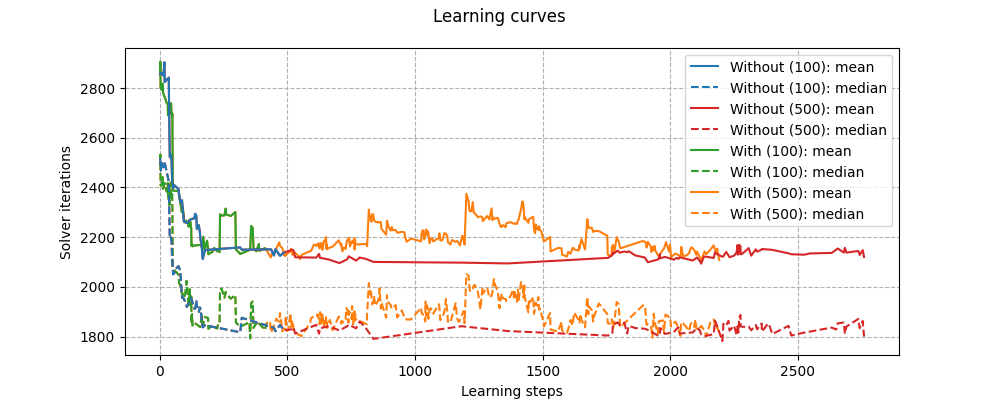
\includegraphics[width=1\textwidth]{plots/disimprove_learn_curve.png}
    \caption{Learning curves for the testing disimprovement where the blue and red lines corresponds to runs without disimprovement with 100 and 500 base learning iterations, this is the same data as in figure \ref{fig: plateau learning curves}, green and orange lines are with disimprovement with 100 and 500 base learning iterations, the new test. Line style corresponds to whole line for the mean and dashed line for the median solver iteration count.}
    \label{fig: disimprove learning curves}
\end{figure}

\begin{figure}[H]
    \center
    \begin{minipage}{.49\textwidth}
        \center
        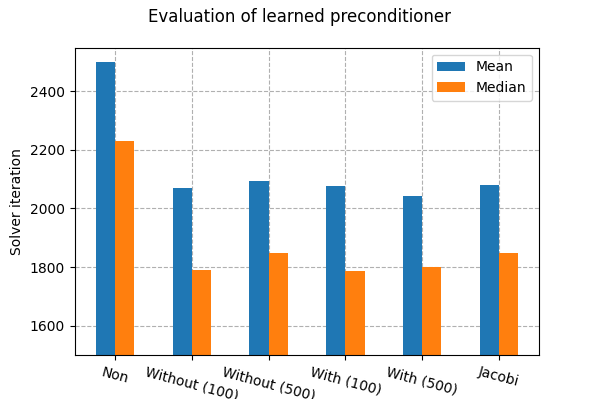
\includegraphics[width=1\textwidth]{plots/disimprove_test_measure.png}
        \caption{Mean and median solver iteration count for the evaluation of the learned preconditioner. Colour indicate measure: Blue is mean and orange is median solver iteration count. A bar group for each of the four tests: without disimprovement with 100 and 500 base learning iterations and with disimprovement with 100 and 500 base learning iteration. On either end the unpreconditioned and Jacobi preconditioned systems for comparison.}
        \label{fig: disimprove test measure}
    \end{minipage}
    \begin{minipage}{.02\textwidth}
        
    \end{minipage}
    \begin{minipage}{.49\textwidth}
        \center
        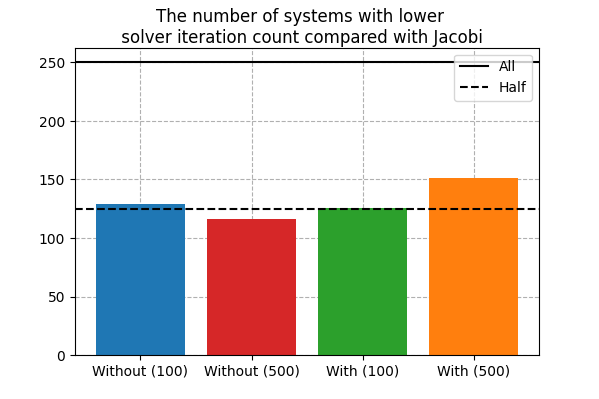
\includegraphics[width=1\textwidth]{plots/disimprove_BvJ.png}
        \caption{Individual linear system comparison between the learned preconditioners and Jacobi preconditioners with bar size corresponding to the number of systems where the learned preconditioner has a lower solver iteration count that Jacobi Preconditioning.\\\\\\}
        \label{fig: disimprove BvJ}
    \end{minipage}
\end{figure}


To resolve this problem the algorithm should keep tack of the best seen preconditioner. Here we would like to again use the improvement function as a measure for which were the best, but the SIGN improvement function can not do comparisons across multiple solver iteration count data sets. Therefore we will use the discarded improvement functions mean and median in combination to determine which accepted preconditioner was the best, as these measure are the measures we look at to determine if the learned preconditioner are good in the evaluation. This measure of best will be done after a new preconditioner have been accepted.

